\section{Design}\label{sec:design}
\subsection{Systemets sammenheng}\label{sec:design:sammenheng}

Systemets informasjonsflyt er illustrert i figur \ref{fig:blokkDig}. 
Det infrarøde kameraet sender en kontinuerlig videostrøm til prosesseringsenheten, som detekterer antall fugler i bildet. 
Prosesseringsenheten skal videre ta inn data fra værsensorene og tolke disse, før dataene sendes videre til en database. 
En nettside skal så hente og vise fram dataen fra databasen, slik at brukeren får et oversiktlig bilde over fugleaktiviteten i området. 

\begin{figure}[H]
    \centering
    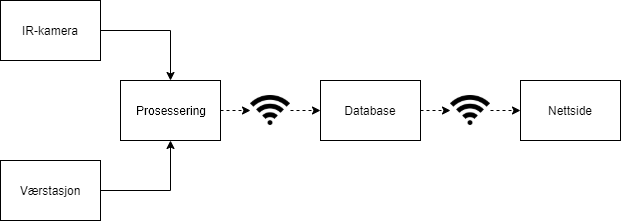
\includegraphics[width=0.9\textwidth]{design/designflytskjema.png}
    \caption{Blokkdiagram over systemet. Fuglene blir detektert av et infrarødt kamera og bildene prosesseres. Værdata samles inn. Data blir så sendt videre til en database og vist fram på en nettside.}
    \label{fig:blokkDig}
\end{figure}

\newpage
\subsection{Systemkrav}\label{sec:design:systemkrav}
Tabell \ref{tab:systemkrav} viser systemkravene. 
Disse er i stor grad basert på at systemet skal stå utendørs ved vindturbinen Vestas v27-225kW \cite{vindturbin}.
Det er denne type vindturbin som står på Rye i Trondheim, og dette området blir brukt som testarena. 




\begin{table}[!htbp]
\centering
\caption{Systemkrav.}
\label{tab:systemkrav}
\resizebox{\textwidth}{!}{%
\begin{tabular}{|l|l|l|}
\hline
\multicolumn{3}{|l|}{\textbf{Generelt}}                                                                             \\ \hline
\textbf{Kravnavn}    & \textbf{Beskrivelse}                                               & \textbf{id}             \\ \hline
Mål                  & Systemet skal detektere og dokumentere fugleaktivitet i luften.    & \idlabel{id:mål}        \\ \hline
Værbestandighet      & Systemet skal være vanntett og tåle å stå ute i norske værforhold. & \idlabel{id:IPrating}   \\ \hline
Strømforsyning       & Systemet vil få strøm fra strømnettet.                             & \idlabel{id:strøm}      \\ \hline
Værdata &
  \begin{tabular}[c]{@{}l@{}}Systemet vil ha temperatur, lufttrykk, luftfuktighet, \\ nedbørmåler og vindsensor.\end{tabular} &
  \idlabel{id:telemetri} \\ \hline
\multicolumn{3}{|l|}{\textbf{Deteksjon}}                                                                            \\ \hline
\textbf{Kravnavn}    & \textbf{Beskrivelse}                                               & \textbf{id}             \\ \hline
Synsvinkel &
  \begin{tabular}[c]{@{}l@{}}Systemet vil bruke et infrarødt kamera med en minimum \\ synsvinkel på $\ang{41}$x$\ang{31}$.\end{tabular} &
  \idlabel{id:kamera} \\ \hline
Rekkevidde           & Systemet skal ha en rekkevidde på minimum 50 meter.                & \idlabel{id:rekkevidde} \\ \hline
Størrelse &
  \begin{tabular}[c]{@{}l@{}}Systemet skal minimum detektere fugler med størrelse \\ ned til 300x100mm innenfor rekkevidden.\end{tabular} &
  \idlabel{id:temperatur} \\ \hline
\multicolumn{3}{|l|}{\textbf{Fysiske dimensjoner}}                                                                  \\ \hline
\textbf{Kravnavn}    & \textbf{Beskrivelse}                                               & \textbf{id}             \\ \hline
Dimensjoner          & Produktet vil være mindre enn 200x300x300mm ekskudert stativ.      & \idlabel{id:størrelse}  \\ \hline
\multicolumn{3}{|l|}{\textbf{Overføring, behandling og fremstilling av data}}                                       \\ \hline
\textbf{Kravnavn}    & \textbf{Beskrivelse}                                               & \textbf{id}             \\ \hline
Prosesseringsenhet   & Dataene vil behandles av en liten ettkortsdatamaskin.              & \idlabel{id:prosessor}  \\ \hline
Programvare          & Programvaren vil være basert på åpen kildekode.                    & \idlabel{id:opensource} \\ \hline
Treffrate\footnotemark &
  \begin{tabular}[c]{@{}l@{}}Programvaren skal være god nok til å detektere minimum\\ 75\% av fuglene innenfor synsvinkelen og rekkevidden til kameraet.\end{tabular} &
  \idlabel{id:treffrate} \\ \hline
Overføring internt &
  \begin{tabular}[c]{@{}l@{}}Systemet vil bruke USB til å overføre data mellom \\ kamera og prosesseringsenhet.\end{tabular} &
  \idlabel{id:internoverføring} \\ \hline
Overføring eksternt &
  \begin{tabular}[c]{@{}l@{}}Systemet vil bruke Wi-Fi for å overføre data fra \\ prosesseringsenhet og databasen.\end{tabular} &
  \idlabel{id:eksternoverføring} \\ \hline
Fremstilling av data & Resultatene vil fremstilles på en nettside.                        & \idlabel{id:nettside}   \\ \hline
\end{tabular}
}
\end{table}
\footnotetext{Antall fugler som er talt og sporet korrekt}

\newpage
\subsection{Kamera}\label{sec:design:kamera}

Et infrarødt kamera (heretter kalt IR-kamera) brukes til å detektere infrarød stråling. 
Infrarød stråling er elektromagnetisk stråling med en bølgelengde mellom $\SI{7}{\micro\meter}$ og $\SI{1}{\milli\meter}$ \cite{SNL-IR}.
Alle objekter med en temperatur mellom det absolutte nullpunkt (0K) og ca 3900K sender ut slik stråling \cite{SNL-IR}, og bølgelengden og intensiteten til denne strålingen kan brukes for å avgjøre temperaturen til objektet. 
I dette designet brukes et IR-kamera for å detektere den infrarøde strålingen emittert fra fugler. 
Fugler er varmblodige og holder en kroppstemperatur på rundt $\SI{40}\:{\degree}$C \cite{snlfugl}.
De emitterer infrarød stråling som i prinsippet kan detekteres av et infrarødt kamera.
Himmelen i bakgrunnen vil oppføre seg som et tilnærmet svart legeme, og dermed emittere en relativt mindre mengde IR-stråling.

Et IR-kamera brukes i stedet for et vanlig kamera, da det gjør det enklere å detektere fuglene mot himmelen. 
Et godt eksempel på dette vil være når en hvit måke flyr foran hvite skyer. 
Fargen til måken vil da kunne gå i ett med skyene, og gjør bildebehandlingen for å detektere fuglen svært vanskelig. 
Med et IR-kamera vil det være mulig å se forskjell på fugler og skyer, og fuglen kan dermed detekteres. 
Videre vil et IR-kamera også gjøre det mulig å detektere fugler når det er mørkt, i motsetning til et konvensjonelt kamera. 
En av ulempene med IR-kamera er at fuglenes fysiske trekk ikke er like synlige, som for eksempel farge, som ville gjort det lettere å bestemme fuglenes art.
Et IR-kamera kan også fungere dårligere i noen værtyper, som regn og snø, da nedbør vil kunne emittere relativt mye IR-stråling, og gi mange falske positiver\footnote{Registrering av fugler som ikke er til stede}.

\subsection{Deteksjon}\label{sec:design:deteksjon}

En prosesseringsenhet skal ta inn en kontinuerlig strøm av bilder fra kameraet og behandle disse bilde for bilde. 
Bildebehandlingen skal finne objekter i bildet, eller såkalte \textit{blobs}\footnote{Forkortelse for Binary Large OBjects}. 
Objektene som skal oppdages er fugler, og disse vil skille seg fra bakgrunnen på grunn av deres høyere temperatur, som representeres ved at de har ulik farge fra bakgrunnen på bildene. 
Bildebehandlingen skal kunne detektere flere objekter i samme bildet. 
I tillegg skal et bilde kunne sammenlignes med forrige bilde for å finne ut om et objekt har beveget seg, og dermed kunne følge dette objektet gjennom en bildeserie. 
Slik unngås det at hver fugl telles en gang per bilde, men blir i stedet fulgt fra den kommer inn i synsvinkelen til kameraet til den går ut, og blir registrert som én fugl.

Dersom systemet plasseres foran en allerede instalert vindturbin, er det ønskelig at deteksjonsområdet minimum dekker området som  vist i \autoref{fig:TurbinForan} og \ref{fig:TurbinSiden}\footnote{Det er ikke nødvendig at kameraet står foran vindturbinen, da den vil rotere for å peke inn i vinden. Vindturbinen er tegnet inn for å vise at deteksjonsområdet ikke skal inneholde turbinen.}.
Videre plasseres kameraet slik at vindturbinen ikke er i synsvinkelen til kameraet, da dette vil kunne forstyrre målingene. Trær, bygginger, kraftlinjer eller andre større objekter,  bør heller ikke være i kameraets synsvinkel. 

%I utgangspunktet skal systemet detektere fugler i området foran vindturbinen (dersom en turbin allerede er installert i området), som er der det vil være størst sannsynlighet for at detekterte fugler vil kollidere med vindturbinen. 
%Deteksjonsområdet ønskes å minst dekke området som er vist i \autoref{fig:TurbinForan} og \ref{fig:TurbinSiden}\footnote{Det er ikke nødvendig at kameraet står foran vindmøllen, da den vil rotere for å peke inn i vinden. Vindmøllen er tegnet inn for å vise at deteksjonsområdet ikke skal inneholde turbinen.}.
%Videre plasseres kameraet slik at vindturbinen ikke er i synsvinkelen til kameraet, da dette vil kunne forstyrre målingene. Trær eller andre større objekter som kraftlinjer bør heller ikke være i kameraets synsvinkel. 

\begin{figure}[!htbp]%hentet fra https://www.cadblocksfree.com/en/wind-turbine.html
  \centering
  \begin{minipage}[b]{0.45\textwidth}
    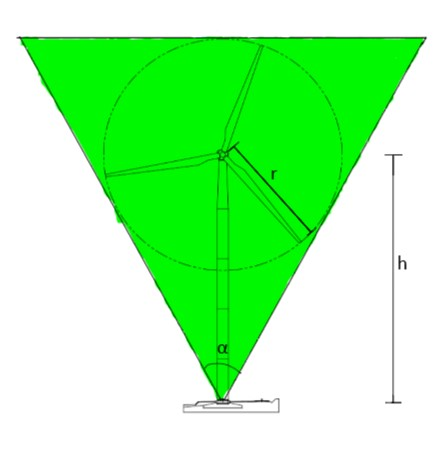
\includegraphics[width=0.8\textwidth]{design/DeteksjonForan.jpg}
    \caption{Deteksjonsområdet til systemet sett fra framsiden av vindturbinen, markert i grønt. }
    \label{fig:TurbinForan}
  \end{minipage}
  \hfill
  \begin{minipage}[b]{0.45\textwidth}
    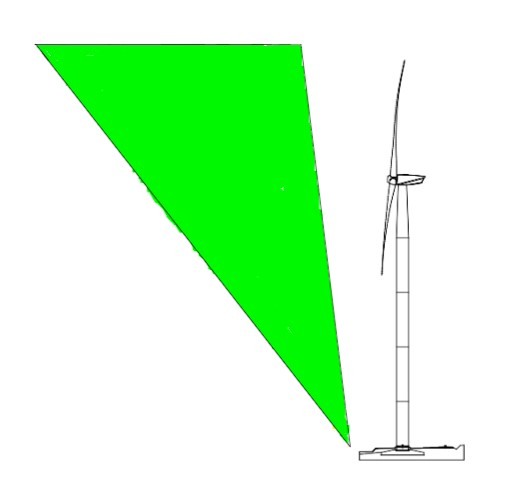
\includegraphics[width=0.8\textwidth]{design/DeteksjonSiden2.jpg}
    \caption{Deteksjonsområdet til systemet sett fra siden av vindturbinen, markert i grønt.}
    \label{fig:TurbinSiden}
  \end{minipage}
\end{figure}

\newpage
\subsection{Værstasjon}\label{sec:design:vaerstasjon}
Systemet skal ha egne sensorer for innsamling av værdata. 
Systemet vil kunne måle temperatur, trykk og fuktighet i lufta, i tillegg til vindhastighet, vindretning og nedbør.
Dataene fra sensorene skal kunne knyttes opp mot fugleaktiviteten, for å finne eventuelle sammenhenger mellom vær og fugleaktivitet. 
Dette kan så brukes til for eksempel å estimere sannsynligheten for at en fugl kolliderer med en vindturbin i ulikt vær og ulike årstider.

\subsection{Nettside og database}\label{sec:design:nettside}

Systemet vil ha en nettside som skal fremstille data som samles fra systemet. 
Data skal vises på en slik måte at den er lett forståelig og navigerbar for en bruker uten spesiell teknisk kompetanse. 
Data skal kunne sorteres etter behov for å se trender i fugleaktivitet, for eksempel time for time eller dag for dag. 
Det vil også være mulig å eksportere rådata direkte fra nettsiden. 

Det blir brukt en database for å lagre data fra værsensorene, kameraet og prosessoren. Det blir tatt utgangspunkt i at det er Wi-Fi dekning der produktet plasseres. Databasen vil brukes som et mellomledd mellom sensorene og nettsiden. Det trengs dermed ikke å skrives en egen protokoll for overføring av data.

\subsection{Strukturelt}\label{sec:design:strukturelt}

Prosesseringsenheten og kameraet skal monteres sammen i en boks, som skal beskytte elektronikken og systemet mot vær og annen ytre påvirkning. 
Boksen skal være festet til en påle for å heves over bakkenivå, slik at forstyrrelser eller skader fra dyr unngås, samt for ikke å tildekkes av snø eller vegetasjon.
Videre skal boksen tilfredsstille systemkrav \idref{id:IPrating} om å være værbestandig, og dimensjonskravene \idref{id:størrelse} fra \autoref{tab:systemkrav}. 
Værsensorene skal være festet på samme påle som resten av systemet. 
Systemet vil få strøm fra det lokale strømnettet.



